\documentclass[11pt]{article}
\usepackage[utf8]{inputenc}
\usepackage[T1]{fontenc}

\usepackage{mathptmx}

\title{Analysing Orphaned Triples in a Large-Scale Graph Database}
\author{Gary Gurlaskie}
\date{15 April 2020}

\usepackage[]{geometry}
\usepackage{natbib}
\usepackage{graphicx}
\usepackage{url}
\usepackage{xcolor}
\usepackage{listings}
\usepackage[parfill]{parskip}
\lstset{basicstyle=\footnotesize\ttfamily,breaklines=true}

\begin{document}

\begin{titlepage}
 \centering
 \vspace*{1in}
 \begin{Large}\bfseries
  Analyzing Orphaned Triples in a Large-Scale Graph Database\par
 \end{Large}

 \vspace*{0.2in}

  CIS4914 -- Final Report\par
  Spring 2020\par

  \vspace*{0.2in}
  
  Gary Gurlaskie (\url{g.gurlask@ufl.edu})\par
  Individual Project\par
  16 April 2020\par
\end{titlepage}

\section*{Abstract}
This project emphasized data analysis and visualization, and was focused on UF VIVO, an 7.1GB RDF graph database that documents UF research efforts. The goal was to identify data in VIVO that had become "orphaned" (disconnected) from the graph.

The analysis was performed ad hoc using Python. Analysis performed included examining zero- or low-degree nodes, connected components, and performing constraint validation against the published ontology.

The work yielded over 10,000 orphaned triples. However, the quality of the data was high overall; 94\% of the graph was connected in a robust way.

\section*{Introduction}
This project was focused on the analysis and visualization of orphaned data in UF VIVO, an 7.1GB graph database that documents UF research efforts. The database is managed by the UF Clinical and Translational Science IT (CTS-IT) and the VIVO application is publicly accessible at \url{vivo.ufl.edu}. This project was selected because it involved working with real-world data on a large scale. This data has been managed by the CTS-IT for years, and they have a number of full- and part-time employees working on the development of the VIVO application. Moreover, this project has a positive impact on data quality (and potentially database performance) for the University of Florida, which makes it desirable to complete as well.

The project mainly involved the application of basic database and graph algorithms (i.e., table scan, indexing, union find) to an RDF database, so the majority of literature surveyed relates to the RDF database itself. RDF databases are essentially composed of two parts: the "triples" and the "ontology". The triples are values of the form "subject, predicate, object", where each element is a URI. These values carry semantic meaning -- for example, one triple may be "n9633259703 has-type person", or more concretely, "<http://vivo.ufl.edu/individual/n9633259703> <http://www.w3.org/1999/02/22-rdf-syntax-ns\#type> <http://xmlns.com/foaf/0.1/Person>".

The ontology introduces both constraints and an inheritance structure on the triples. Readers familiar with object-oriented programming may find this similar to the Java programming language. Different ontologies are typically combined to form the "schema" for the composite database -- for example, the VIVO ontology uses the FOAF ("friend of a friend"), OBO ("Open Biological and Biomedical Ontology") and VCARD ontologies, and introduces additional classes such as "vivo:Authorship", which relates a "foaf:Agent" and an "obo:InformationContentEntity" (a generic class whose subclasses include "bibo:article" or "obo:TextualEntity"). Relations such as "vivo:Authorship" can carry additional metadata, such as dates. "vivo:Authorship" also carries constraints, such as that it must include at least one "vivo:relates" edge to a "foaf:Agent" and at least one "vivo:relates" edge to an "obo:InformationContentEntity".

The data analyzed was in N-Quads format, which is an unordered list of all the triples in the form "subject, predicate, object, graph". The "graph" parameter is used to combine multiple RDF databases into a single N-Quads file, and was not used for this project. The N-Quads format is designed to be "easy to parse".

\section*{Solution}
In this project, we produced a collection of tuples that we defined to be orphaned. This involved software components and data analysis components. The software was executed on a 2015 MacBook Pro, so we needed to take a stream processing approach to manipulate the 7.1GB N-Quads file. For the analysis, three approaches employed were successful in screening for orphaned triples.

\subsubsection*{Stream Processing}
We determined that processing the N-Quads file as a stream was the most efficient approach to run our queries. There are a number of reasons for this. First, the file contained 37,983,245 triples and was 7.1GB -- not feasible to load into memory. Additionally, loading the file into a SQLite database may seem promising, we are mainly interested in the global properties of the data, so most queries would require a full table scan. Moreover, we wanted to perform complex aggregations, such as determining connected components, which are not possible to express in a SQL query.

Parsing the N-Quads file was extremely simple. Each line is a space-separated array of four URIs enclosed in angle brackets ("<uri> <uri> <uri> <uri> ."). We are only interested in the first three URIs. Therefore, we simply have to look for the first three spaces and split the string into subject, predicate, and object. This was accomplished using native Python.

We also parallelized similar queries. Reading, parsing, and iterating through the file takes a large amount of processing time. To perform schema validation, we needed to run 23 similar queries on a full scan. Instead of scanning through the triples 23 times, we found it much more performant to run the queries in parallel -- the triples are scanned through once, and each query consumes the current triple before moving onto the next. This enabled the entire constraint-checking to run on the order of a few minutes.

Finally, although there were 30 million lines, there were only a few million entities, so we precomputed useful information, such as the type(s) of each entity and the number of edges.

\subsubsection*{Analysis}
The first approach was a naive definition of orphaning -- we wanted to determine which entities had no neighbors. For this, we ignored predicates and used a regular expression to match VIVO entities. We defined that VIVO entity A is has neighbor B if there is an edge such that A <predicate> B or B <predicate> A, regardless of the actual predicate. 

\section*{Results}

\section*{Conclusions}

\section*{Standards}

\section*{Constraints}

\begin{lstlisting}
a := 1;
\end{lstlisting}

\begin{figure}[h!]
\centering
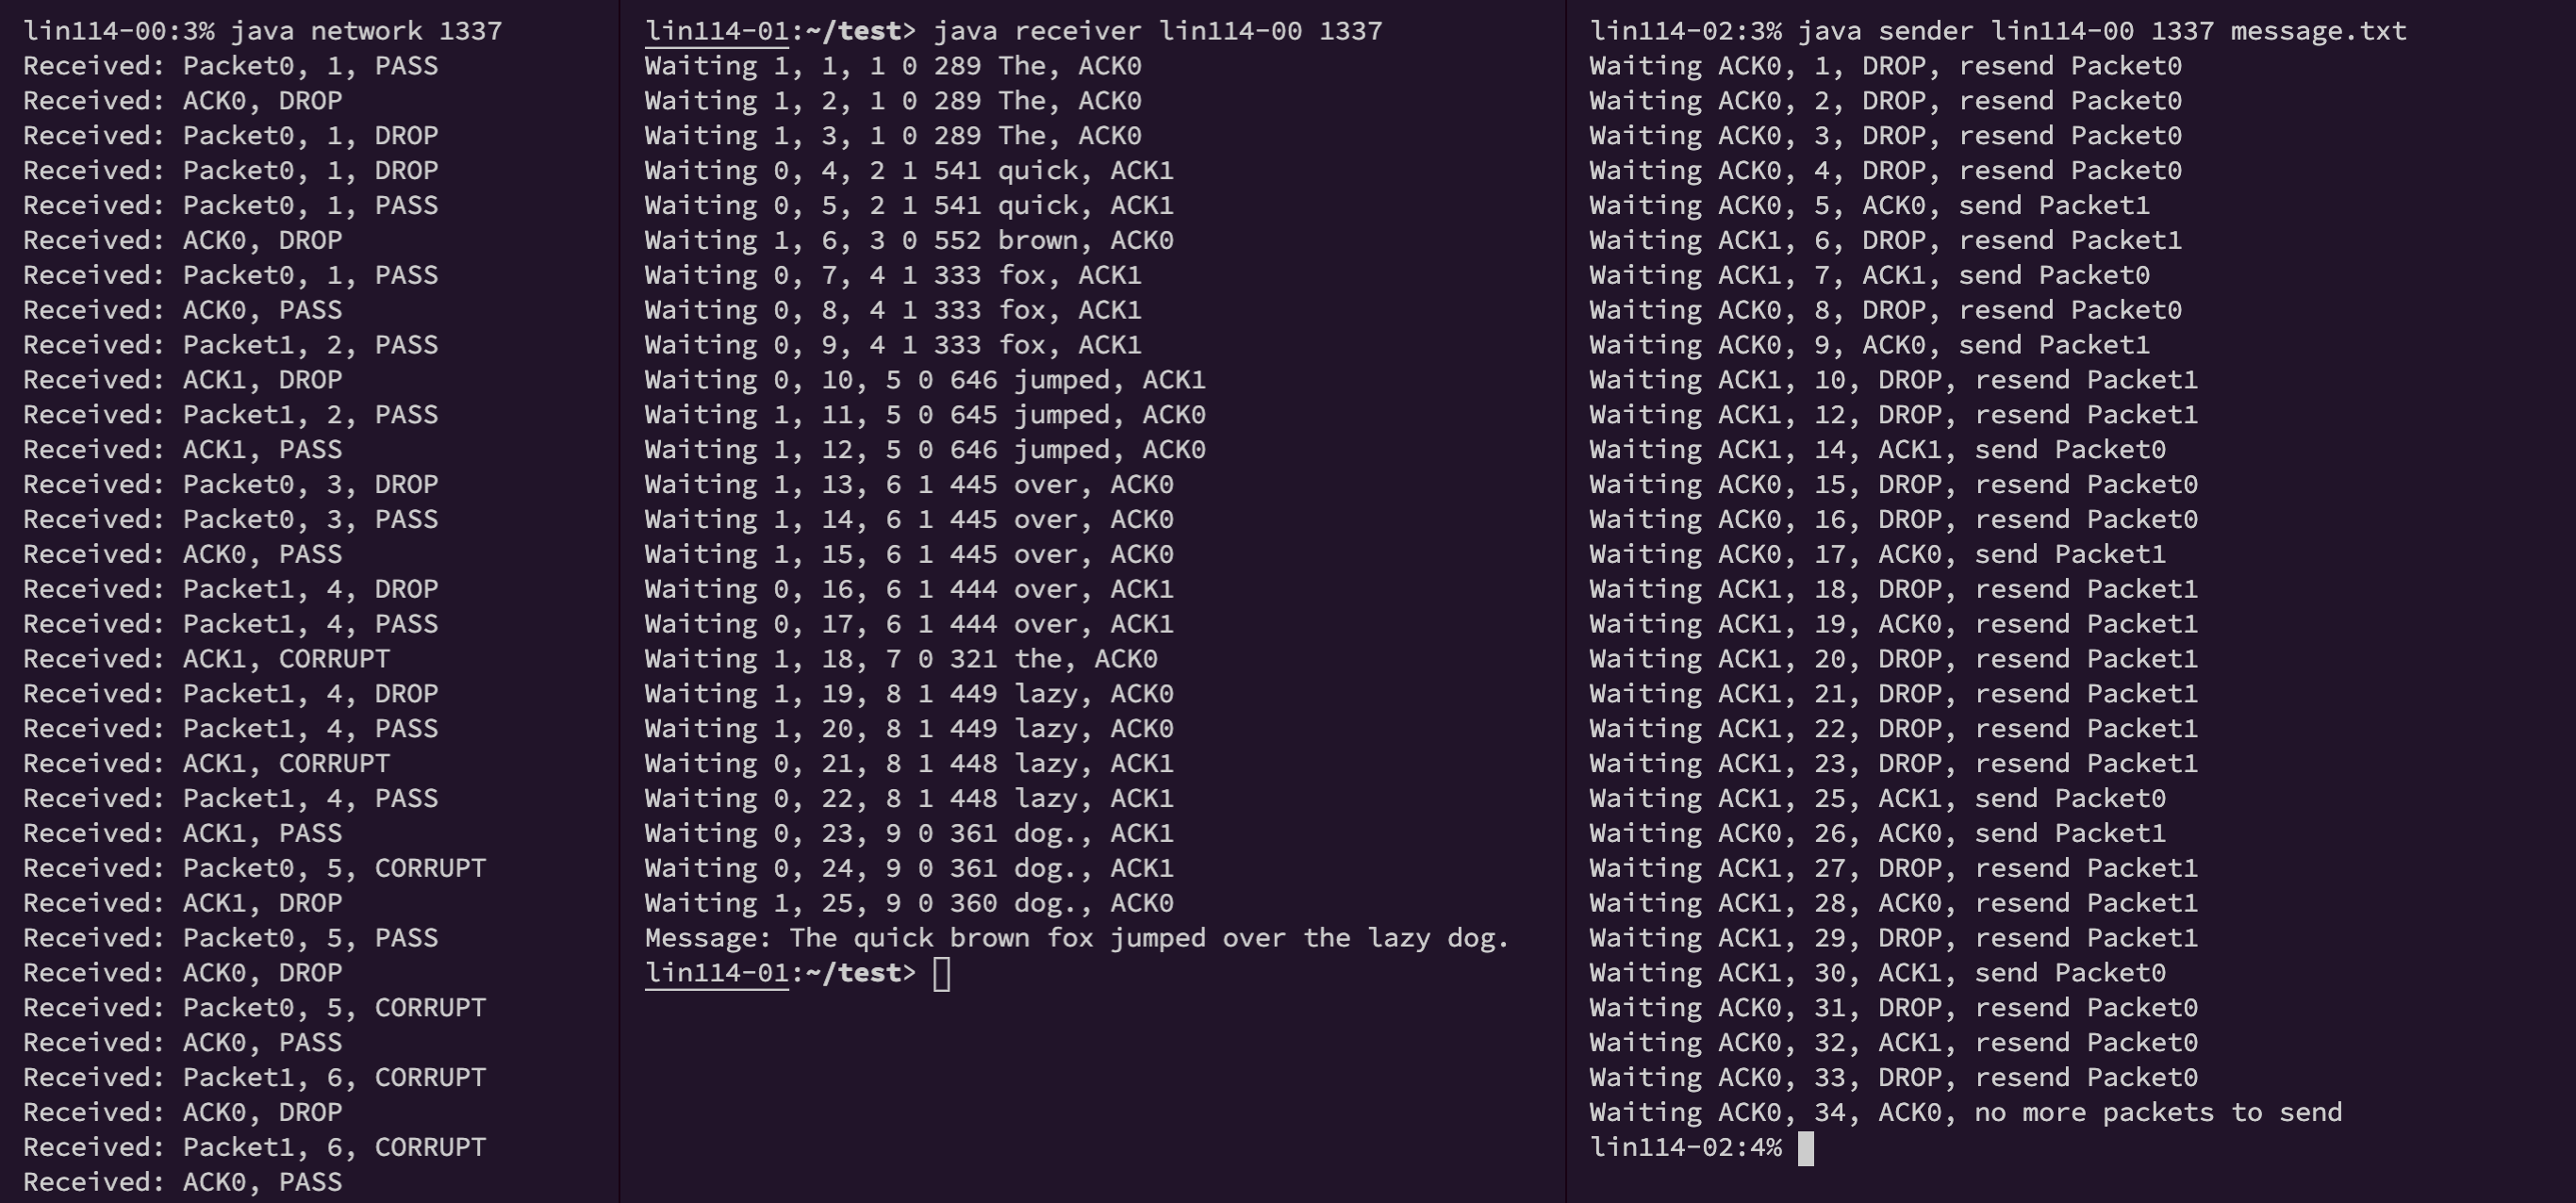
\includegraphics[width=\textwidth]{output.png}
\caption{An example execution.}
\label{fig:output}
\end{figure}

\section*{Acknowledgments}
The author thanks Christopher Barnes for advising the project, and the UF CTS-IT for providing access to the VIVO data. The author also thanks Taeber Rapczak for his excellent help and guidance.

\section*{References}
[RDF] Ora Lassila and Ralph Swick. “Resource Description Framework (RDF) Model and Syntax Specification”, https://www.w3.org/TR/1999/REC-rdf-syntax-19990222, W3C (as-of 6 April 2020).

[NQuads] Gavin Carothers and Lex Machina, Inc. “RDF 1.1 N-Quads: A line-based syntax for RDF datasets”, https://www.w3.org/TR/n-quads/, W3C (as-of 6 April 2020).

[OWL] Mike Dean, et al. "OWL Web Ontology Language", https://www.w3.org/TR/owl-ref/, W3C (as-of 15 April 2020).

[Python] Guido van Rossum. “The Python Programming Language”, https://python.org, Python Software Foundation (as-of 6 April 2020).

\section*{Biography}
Gary Gurlaskie is an undergraduate student studying Mathematics and Computer Science at the University of Florida. He worked at Ultimate Software (data platform engineering) and Intel (software engineering). He plans to graduate in May 2020, and upon graduation will move to Portland to work at Intel full-time. He has always wanted to have a cat, so he will obtain one when he moves to Oregon.

\end{document}

